\section{Results}

\subsection{360 scan}

When the robot was placed on the center of the arena, it could always find the entrance to the room it wanted to navigate to, no matter its initial orientation.

When the robot was started, during the initial 360 scan, it turned on itself clockwise, using the IR sensors to sense its surroundings.\\
The procedure responsible for the 360 scan waited for both sensors to be higher than a threshold of 180, and identified that as being the only wall that could be perpendicular to the direction the robot was facing. After that, it counted the number of gaps with the left sensor and stopped on the gap of the room of interest.

\begin{figure}[ht]
    \centering
    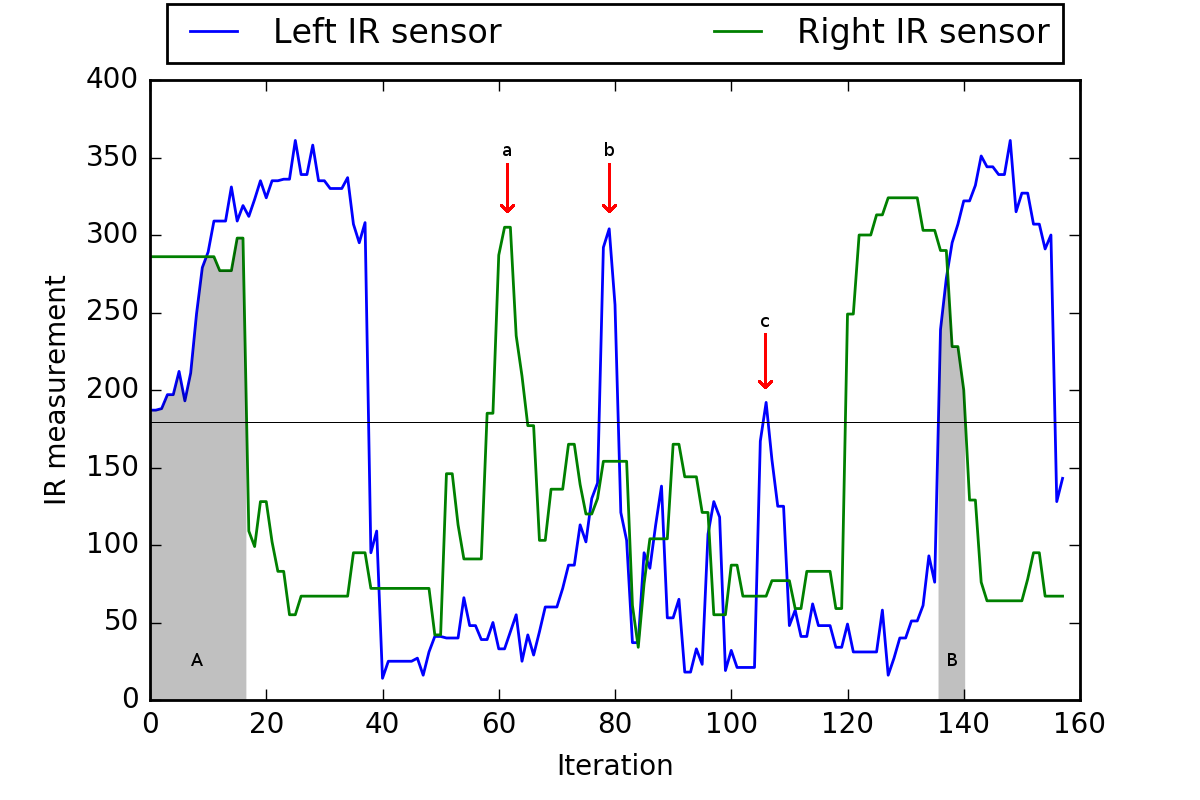
\includegraphics[width=0.7\linewidth]{res/360-scan-plot.png}
    \caption{Samples of the IR sensors while performing a 360 scan at home (the center of the arena). (A) and (B) are the moments when both sensors are triggered past the threshold, i.e., the robot is perpendicularly facing the wall of the center of the arena. (a) and (b) are the moments the right and left sensor pass by the edge of the wall between the entrance for room B and room A, respectively. (c) is when the left sensor passes by the edge of the wall between room A and room C (the smallest of the rooms).}
\end{figure}

% - - - - - - - - - - - - - - - - - - - - - - - - - - -

\newpage
